\subsection{Source-Degenerated (SD) CTLE}

The source-degenerated (SD) CTLE is the most widely adopted active equalization topology in high-speed serial link receivers, including PCIe SerDes PHYs. Compared to passive CTLEs, the SD CTLE provides \textbf{true high-frequency gain} by exploiting the transistor transconductance while maintaining relatively low complexity and power consumption.Unlike passive equalizers that rely solely on frequency-dependent attenuation, the SD CTLE actively reshapes the frequency response by introducing a \emph{frequency-dependent source degeneration impedance}. This enables controlled peaking, wider equalization range, and tunability across different channel conditions.

\subsubsection*{Circuit Architecture}

Figure~\ref{fig:sd_ctle_arch} illustrates the conventional SD-CTLE topology, which consists of a differential transconductance stage with resistive loads $R_L$, and a source degeneration network composed of resistor $R_s$ and capacitor $C_s$ connected at the common-source node.

\begin{figure}[H]
    \centering
    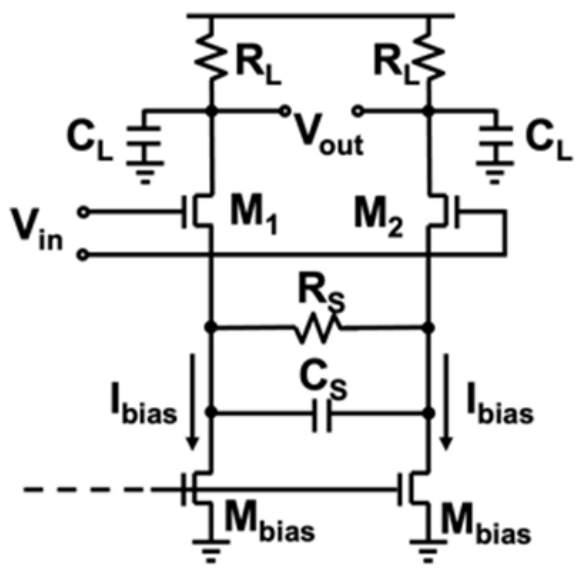
\includegraphics[width=0.35\textwidth]{img/CTLE_img/SD CTLE schematic.png}
    \caption{Conventional source-degenerated CTLE circuit architecture.}
    \label{fig:sd_ctle_arch}
\end{figure}

The differential pair transistors $M_1$ and $M_2$ convert the input voltage $V_{in}$ to a current, while the degeneration network modulates their effective transconductance as a function of frequency. The bias current $I_{bias}$ sets the operating point and transconductance $g_m$ of the input pair. The key innovation of this topology is the placement of $C_s$ in parallel with $R_s$: at low frequencies, $C_s$ is effectively open-circuited, making the degeneration impedance primarily resistive ($R_s$); at high frequencies, $C_s$ shorts out $R_s$, reducing degeneration and thereby boosting the gain. This frequency-selective feedback forms the basis of the CTLE's equalization capability.

\subsubsection{Small-Signal Transfer Function}

The small-signal transfer function of the source-degenerated CTLE is derived using the differential half-circuit model. Each side of the differential pair contributes a transconductance of $g_{m1,2}$, while the source degeneration resistor $R_s$ is shared between the two transistors. As a result, the effective degeneration seen in the half-circuit is $R_s/2$.

\begin{figure}[H]
    \centering
    \begin{minipage}{0.48\textwidth}
        \centering
        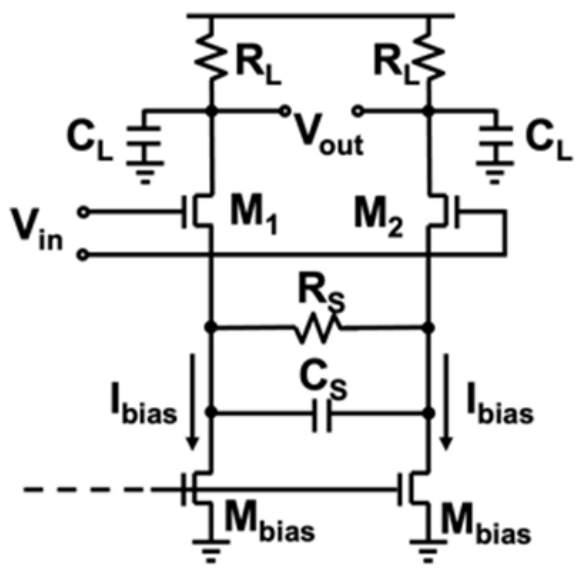
\includegraphics[width=0.7\textwidth]{img/CTLE_img/SD CTLE schematic.png}
        \caption{SD-CTLE circuit schematic.}
        \label{fig:sd_ctle_schematic}
    \end{minipage}
    \hfill
    \begin{minipage}{0.48\textwidth}
        \centering
        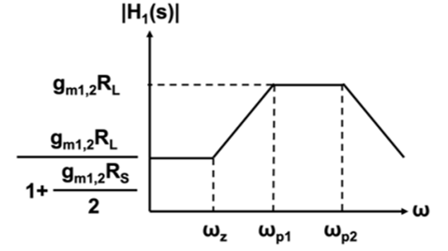
\includegraphics[width=\textwidth]{img/CTLE_img/SD CTLE BEHAV.png}
        \caption{SD CTLE Frequency response.}
        \label{fig:sd_ctle_response}
    \end{minipage}
\end{figure}

The SD-CTLE transfer function, including source degeneration and output loading, is:

\[
\begin{aligned}
H_1(s) = -A_{DC} \cdot \frac{1 + \frac{s}{\omega_z}}{(1 + \frac{s}{\omega_{p1}})(1 + \frac{s}{\omega_{p2}})}, &\quad A_{DC} = \frac{g_{m1,2}R_L}{1 + \frac{g_{m1,2}R_s}{2}}
\end{aligned}
\]

At high frequencies, $C_s$ shorts $R_s$, giving peak gain:
\[
A_{\text{peak,ideal}} = g_{m1,2}R_L
\]
The zero and pole locations are:

\[
\begin{aligned}
\omega_z  &= \frac{1}{R_s C_s}, &\quad
\omega_{p1} &= \frac{1 + \frac{g_{m1,2} R_s}{2}}{R_s C_s}, &\quad
\omega_{p2} &= \frac{1}{R_L C_L}
\end{aligned}
\]

The gain boost, defined as $\frac{A_{\text{peak,ideal}}}{A_{DC}}$, becomes:

\[
\text{Gain Boost} = \frac{\omega_{p1}}{\omega_z} = 1 + \frac{g_{m1,2} R_s}{2}
\]

As shown in Figure~\ref{fig:sd_ctle_response}, $\omega_z$ and $\omega_{p1}$ create the peaking needed for high-frequency compensation, while $\omega_{p2}$ limits bandwidth. The $\omega_{p1}/\omega_z$ ratio, controlled by $g_mR_s$, determines equalization strength.

\subsubsection{Design Knobs and Tunability}
\label{sec:design_knobs}

The SD-CTLE offers four tuning parameters—$R_L$, $R_s$, $C_s$, and $I_{bias}$—for electronic optimization across channel conditions.

\subsubsection*{Effect of Load Resistance $R_L$}
\label{subsec:effect_rl}

The load resistance $R_L$ controls DC gain and bandwidth through $\omega_{p2} = 1/(R_LC_L)$. Increasing $R_L$ boosts gain but reduces bandwidth, establishing the gain-bandwidth trade-off.

\begin{figure}[H]
    \centering
    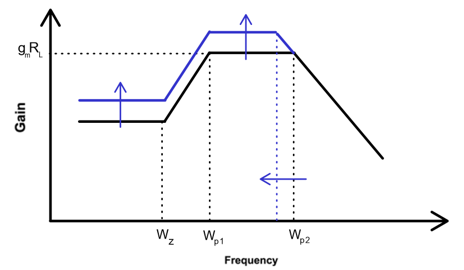
\includegraphics[width=0.55\textwidth]{img/CTLE_img/effect of inc RL.png}
    \caption{Frequency response variation with increasing load resistance $R_L$.}
    \label{fig:effect_rl}
\end{figure}

The effect of increasing $R_L$ can be summarized as:

\begin{itemize}
    \item \textbf{DC Gain Enhancement}: $A_{DC}$ increases linearly with $R_L$, providing higher overall signal amplification.
    \item \textbf{Bandwidth Reduction}: $\omega_{p2}$ decreases inversely with $R_L$, creating a fundamental gain-bandwidth trade-off.
    \item \textbf{Peak Frequency Shift}: While $\omega_z$ and $\omega_{p1}$ remain unaffected by $R_L$, the reduced $\omega_{p2}$ causes the apparent peaking frequency to shift downward as the high-frequency roll-off occurs earlier.
    \item \textbf{Output Swing Increase}: Larger $R_L$ yields higher output voltage swing for a given output current, improving signal-to-noise ratio at the cost of reduced bandwidth.
\end{itemize}

\subsubsection*{Effect of Degeneration Resistance $R_s$}
\label{subsec:effect_rs}

The degeneration resistance $R_s$ represents the most critical tuning knob for controlling the peaking magnitude in SD-CTLE. Unlike $R_L$, $R_s$ affects both the DC gain and the relative spacing between $\omega_z$ and $\omega_{p1}$, thereby directly controlling the gain boost.

\begin{figure}[H]
    \centering
    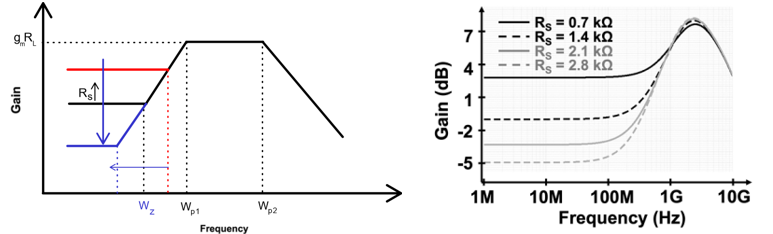
\includegraphics[width=.8\textwidth]{img/CTLE_img/effect of inc RS.png}
    \caption{Frequency response variation with increasing $R_s$: (left) asymptotic response showing ideal behavior; (right) actual response in 180nm technology.}
    \label{fig:effect_rs}
\end{figure}

From the transfer function analysis:
\[
\begin{aligned}
A_{DC} &= \frac{g_{m1,2}R_L}{1 + \frac{g_{m1,2}R_s}{2}}, &\quad
\text{Gain Boost} &= 1 + \frac{g_{m1,2} R_s}{2}, \\
\omega_z &= \frac{1}{R_s C_s}, &\quad
\omega_{p1} &= \frac{1 + \frac{g_{m1,2} R_s}{2}}{R_s C_s}
\end{aligned}
\]

Increasing $R_s$ produces the following effects:

\begin{itemize}
    \item \textbf{Gain Boost Increase}: The gain boost factor grows linearly with $R_s$, enabling stronger high-frequency emphasis.
    \item \textbf{DC Gain Reduction}: $A_{DC}$ decreases as $R_s$ increases, creating an inverse relationship between low-frequency gain and high-frequency peaking.
    \item \textbf{Zero-Pole Spreading}: Both $\omega_z$ and $\omega_{p1}$ shift to lower frequencies, but $\omega_{p1}$ moves more significantly, increasing the $\omega_{p1}/\omega_z$ ratio.
    \item \textbf{Peaking Frequency Reduction}: The frequency of maximum peaking shifts downward, which can be advantageous for compensating channels with attenuation maxima at specific frequencies.
\end{itemize}

\subsubsection*{Effect of Degeneration Capacitance $C_s$}
\label{subsec:effect_cs}

The degeneration capacitance $C_s$ primarily controls the frequency location of the zero $\omega_z$ and the first pole $\omega_{p1}$, thereby setting the frequency range over which gain boosting occurs. While $R_s$ controls \textit{how much} boost, $C_s$ controls \textit{where} the boosting happens.

\begin{figure}[H]
    \centering
    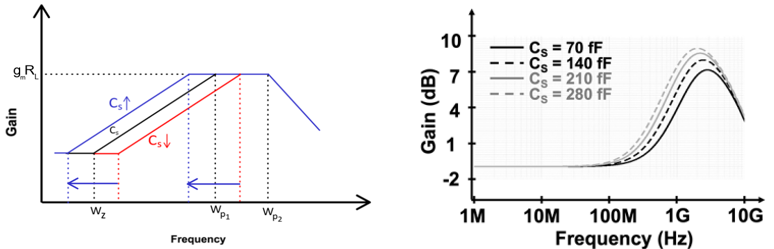
\includegraphics[width=.8\textwidth]{img/CTLE_img/effect of inc CS.png}
    \caption{Frequency response variation with increasing $C_s$: (left) asymptotic ideal response; (right) actual response in 180nm technology.}
    \label{fig:effect_cs}
\end{figure}

The relevant equations governing $C_s$ effects are:
\[
\begin{aligned}
\omega_z &= \frac{1}{R_s C_s}, &\quad
\omega_{p1} &= \frac{1 + \frac{g_{m1,2} R_s}{2}}{R_s C_s}, &\quad
\text{Gain Boost} &= 1 + \frac{g_{m1,2} R_s}{2}
\end{aligned}
\]

Key observations for increasing $C_s$:

\begin{itemize}
    \item \textbf{Frequency Scaling}: Both $\omega_z$ and $\omega_{p1}$ decrease proportionally with $C_s$, maintaining their ratio constant.
    \item \textbf{Constant Gain Boost}: Unlike $R_s$, varying $C_s$ does not alter the gain boost magnitude since it depends only on $g_mR_s$.
    \item \textbf{Peaking Frequency Shift}: The entire peaking profile shifts to lower frequencies, useful for targeting specific channel notches or adjusting to different data rates.
    \item \textbf{Bandwidth Preservation}: The high-frequency roll-off determined by $\omega_{p2}$ remains unchanged, preserving the ultimate bandwidth limit.
\end{itemize}


\subsubsection*{Effect of Bias Current $I_{bias}$}
\label{subsec:effect_ibias}

The bias current $I_{bias}$ controls the transconductance $g_m$ of the input differential pair, providing global gain control while affecting multiple aspects of the frequency response. This parameter offers a power-performance trade-off knob.

\begin{figure}[H]
    \centering
    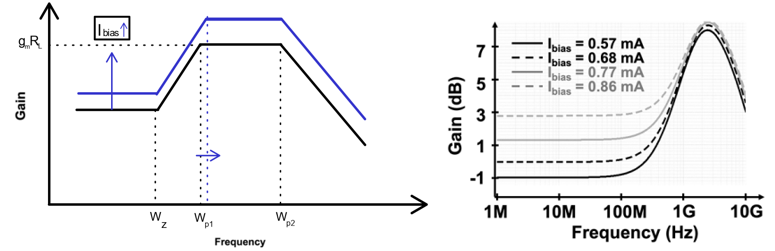
\includegraphics[width=.8\textwidth]{img/CTLE_img/effect of inc ibias.png}
    \caption{Frequency response variation with increasing $I_{bias}$: (left) asymptotic ideal response; (right) actual response in 180nm technology.}
    \label{fig:effect_ibias}
\end{figure}

The transconductance $g_m$ relates to bias current through the square-law approximation for MOSFETs in saturation: $g_m = \sqrt{2\mu_n C_{ox} \left(\frac{W}{L}\right) I_{bias}}$

The circuit parameters affected by $I_{bias}$ (via $g_m$) are:
\[
\begin{aligned}
A_{DC} &= \frac{g_{m1,2}R_L}{1 + \frac{g_{m1,2}R_s}{2}}, &\quad
\omega_{p1} &= \frac{1 + \frac{g_{m1,2} R_s}{2}}{R_s C_s}, &\quad
\text{Gain Boost} &= 1 + \frac{g_{m1,2} R_s}{2}, &\quad
g_m &\propto \sqrt{I_{bias}}
\end{aligned}
\]

Increasing $I_{bias}$ produces these effects:

\begin{itemize}
    \item \textbf{Overall Gain Increase}: Both $A_{DC}$ and peak gain increase with higher $g_m$, though with diminishing returns due to the $\sqrt{I_{bias}}$ relationship.
    \item \textbf{Gain Boost Enhancement}: The gain boost factor increases with $g_m$, providing stronger high-frequency emphasis at higher bias currents.
    \item \textbf{Pole Frequency Shift}: $\omega_{p1}$ increases slightly with $g_m$, while $\omega_z$ remains constant, causing mild peaking frequency upward shift.
    \item \textbf{Power Consumption Trade-off}: Higher $I_{bias}$ directly increases power consumption, making this an important optimization parameter for power-constrained applications.
    \item \textbf{Noise Performance}: Increased $g_m$ generally improves input-referred noise but at the cost of higher power.
\end{itemize}


\subsubsection{Design Trade-offs for the SD CTLE}
\label{subsec:design_tradeoffs}

The interplay between the four primary design knobs creates a multi-dimensional optimization space. Table~\ref{tab:design_knobs_summary} summarizes their effects and typical design considerations.

\begin{table}[H]
\centering
\begin{tabular}{ >{\raggedright\arraybackslash}p{0.12\textwidth} 
                 >{\raggedright\arraybackslash}p{0.23\textwidth} 
                 >{\raggedright\arraybackslash}p{0.25\textwidth} 
                 >{\raggedright\arraybackslash}p{0.30\textwidth} }
\toprule
\textbf{Parameter  } & \textbf{Primary Effect} & \textbf{Secondary Effects} & \textbf{Design Consideration} \\
\midrule
$R_L$ 
    & Controls DC gain 
    & Reduces $\omega_{p2}$, limits bandwidth 
    & Sets fundamental gain-bandwidth trade-off \\
\midrule
$R_s$ 
    & Sets gain boost magnitude 
    & Reduces $A_{\text{DC}}$, lowers $\omega_z$ and $\omega_{p1}$ 
    & Determines equalization strength \\
\midrule
$C_s$ 
    & Positions $\omega_z$ and $\omega_{p1}$ 
    & Shifts peaking frequency 
    & Aligns boosting with channel characteristics \\
\midrule
$I_{\text{bias}}$ 
    & Controls $g_m$ and overall gain 
    & Increases power, affects $\omega_{p1}$ 
    & Power-performance optimization knob \\
\bottomrule
\end{tabular}
\caption{Summary of SD-CTLE Design Knobs and Their Effects}
\label{tab:design_knobs_summary}
\end{table}

